\newpage
\thispagestyle{sectioned}
\chapter{Metodología del Proyecto}

\section{Uso de Software Libre}

\section{Metodología de Migración de Wave a Android}

	\subsection{Objetivo}
  
    El framework de SwellRT utiliza un servidor WIAB y el protocolo Wave, ambos desarrollados en Java. El \textbf{SDK de Android} \cite{ref:android_sdk} es compatible con Java, así que a priori la implantación del servidor no supone problemas en los dispositivos móviles. Sin embargo, existe un problema con el API de SwellRT, ya que el lado del cliente fue desarrollado en Javascript usando el framework GWT. Android no soporta de forma nativa estas tecnologías, así que es necesario estudiar el código de SwellRT para sustituir todo el código que haga uso de Javascript/GWT por código compatible con Android. El objetivo de esta parte del proyecto es conseguir que un cliente desplegado en Android sea capaz de conectarse e interactuar con un servidor Wave sin problemas.  
  
  \subsection{Plataforma: Entorno de Desarrollo, Construcción y Depuración}
  
    Existen dos entornos de desarrollo (IDE) recomendados por Google para desarrollar en Android: Eclipse \cite{ref:eclipse} y Android Studio.\cite{ref:android_studio} Eclipse es un entorno de desarrollo genérico que, mediante plugins, permite extender sus funcionalidades para desarrollar en diversas plataformas y lenguajes. Android Studio es un IDE basado en el entorno de desarrollo Java IntelliJ IDEA \cite{ref:intelliJ_Idea} adaptado para trabajar con todas las funcionalidades de Android. En el momento de empezar con la migración Android Studio se encuentra en fase beta de desarrollo, pues Google pretende convertirla en el IDE de desarrollo oficial para Android. Mientras no se lanza la version final de Android Studio, Google recomienda utilizar Eclipse para desarrollar en Android, y las guias para desarrolladores Android estan escritas para Eclipse. En consecuencia tomamos la decision de utilizar el entorno de desarrollo Eclipse para la migracion de SwellRT a Android. 

    		\subsubsection{Eclipse} \label{sssec:eclipse}
    
    El IDE de Eclipse \cite{ref:eclipse} soporta el desarrollo con Android a través del plugin \textbf{ADT (Android Development Tools)} \cite{ref:eclipse_adt}, que integra en un solo paquete todas las herramientas necesarias para desarrollar, construir y depurar el código de la aplicacion fácilmente. \\[.2cm]
    
    \textbf{Android SDK} \cite{ref:android_sdk}: paquete que integra el conjunto de herramientas necesarias para desarrollar en Android.  Entre estas herramientas destacan las siguientes:
    
    \begin{itemize}
    \item \textbf{Librerías con el API} de Android y \textbf{Documentación} asociada \cite{ref:android_api_reference}
    
    \item \textbf{Android Virtual Device Manager (AVDM)} \cite{ref:android_vdm} herramienta para gestionar la creación, modificación, ejecución y eliminación de emuladores en Android. Un \textbf{emulador} \cite{ref:android_emulator} es una máquina virtual que ejecuta una determinada versión de Android. Permite desplegar un dispositivo movil en el ordenador que imita las características software y hardware de uno real para poder hacer pruebas de desarrollo sin necesidad de poseer un dispositivo con Android. 
    
    \item \textbf{Android SDK Manager} \cite{ref:android_sdk_manager} herramienta para gestionar las versiones de SDK y herramientas asociadas instaladas. Android se encuentra actualmente en la versión 5.1 (API 22), pero un desarrollador puede elegir desarrollar para una versión anterior si lo estima necesario, por lo que puede descargarse por separado dicha versión y mantener varias API si lo necesita.
    
    \item \textbf{Dalvik Debug Monitor Server (DDMS)} \cite{ref:android_ddms} herramienta que provee las características de entorno de depuración para las aplicaciones en desarrollo.

    \end{itemize}
	
	Teniendo en cuenta la distribucion actual de versiones instaladas en dispositivos Android \cite{ref:android_dist} (Ver figura \ref{fig:android_Usage}) se ha decidido realizar la migración de SwellRT con el API 19 de Android (Version 4.4 "KitKat"). El emulador desplegado para las pruebas de desarrollo utilizará por tanto Android 4.4 .

	\begin{figure}[H]
      \centering
	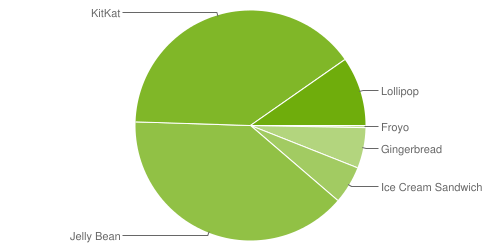
\includegraphics[keepaspectratio, scale=0.8]{Media/Captures/androidUsage.png}
      \caption{Distribución Actual de Versiones Android (Fuente: Google)}
      \label{fig:android_Usage}
    \end{figure}

	Sin embargo existe un problema con la construcción y depuración del código de SwellRT en Eclipse. Android \textbf{limita el número de métodos máximos de una aplicacion a 65K} \cite{ref:android_limit65k} por cuestiones de eficiencia. Para evitar esta limitación, durante el proceso de construcción el SDK de Android utiliza, entre otras, una herramienta llamada \textbf{ProGuard} \cite{ref:android_proguard}. Esta herramienta se encarga de optimizar el código de la aplicacion buscando remover clases que no se utilizan y ofuscando el código para prevenir la ingeniería inversa. En el caso de SwellRT, el código posee un gran número de clases java necesarias para desplegar el servidor y el cliente de la herramienta, por lo que es necesaria dicha optimización de código realizada por ProGuard. El sistema de compilación de aplicaciones de Android tiene dos formas: compilacion de la aplicacion en modo debug (para hacer pruebas cuando todavía se encuentra en fase de desarrollo) y en modo release (la aplicación se encuentra en su versión final y se empaqueta y se firma digitalmente para lanzarla al público). En el caso de Eclipse, ProGuard solo se ejecuta cuando se construye en modo release, por lo que cuando se intenta compilar una aplicación con tantas clases como SwellRT mientras se desarrolla (modo debug) el sistema da error y no se puede compilar el código para probarlo en el emulador. \\[.2cm]

	La solución que encontramos fue desarrollar en Eclipse (por las facilidades que el entorno proporciona para escribir código) pero realizar el proceso de construcción del código por consola de comandos, ya que en este caso sí que se puede compilar la aplicación en modo debug utilizando ProGuard.

	     
    		\subsubsection{Proceso de Construcción por Consola}

		Para construir la aplicación por consola de comandos, Android utiliza la herramienta Apache Ant \cite{ref:ant} para automatizar el proceso de construcción \cite{ref:android_cmd_line}. Es importante asimismo tener definida la variable de entorno JAVA\_HOME con la ruta de acceso al JDK de java instalado en la máquina. Conviene también, por comodidad a la hora de trabajar con la consola, añadir al PATH del sistema las rutas a la carpeta donde esta el SDK de android (/sdk) y dentro de esta ruta añadir asimismo rutas a las carpetas /tools y /platform-tools. \\[.2cm]

Existen dos formas de realizar la construcción en modo debug de una app: \\[.2cm] 

\textbf{1 - Sin tener previamente lanzado un emulador o conectado al ordenador un dispositivo android en modo debug \cite{ref:android_device_setUp}:} \\[.2cm]
 
 	 En este caso es necesario construir la aplicación y luego lanzar el emulador para después instalar la aplicación en él. Para construir la aplicacion en modo debug nos vamos a la carpeta raíz de nuestro proyecto y ejecutamos el siguiente comando: 

 	 \begin{lstlisting}[style=console, numbers=none]
		$ ant clean debug
	 \end{lstlisting}
 	 
 	 Esto nos generará una aplicacion instalable en el directorio /bin del proyecto bajo el formato que Android usa para sus aplicaciones (.apk). El siguiente paso es ejecutar un emulador o conectar un dispositivo android por USB. Para ejecutar un emulador, abrimos otra consola y utilizamos el siguiente comando:
 	 
 	 \begin{lstlisting}[style=console, numbers=none]
		$ android avd
	 \end{lstlisting}
 	 
 	 Lo que nos despliega la herramienta Android Virtual Device Manager (Ver Seccion \ref{sssec:eclipse}) para que elijamos/creemos el emulador que queremos ejecutar. Podemos elegir multitud de parámetros \cite{ref_android_avd_params} para el dispositivo que emula (resolución y tamaño de pantalla, de memoria Ram, elementos hardware emulados, etc.) siendo lo más importante elegir un API (versión de Android) que se corresponda con el API que hemos elegido para nuestra aplicación (en nuestro caso API 19). Es recomendable también elegir una imagen del sistema que use un procesador con arquitectura Intel x86, ya que si elegimos la opción por defecto de ARM (los dispositivos móviles actuales usan procesadores ARM) la ejecución del emulador se ralentiza mucho al tener que emular una arquitectura de procesador distinta a la suya (los ordenadores actuales usan arquitectura Intel x86 en su mayoría). Esto únicamente afecta al rendimiento del emulador, la aplicación es independiente de la arquitectura que haya por debajo. \\[.2cm]
 
     Una vez lanzado el emulador/dispositivo móvil, procedemos a instalar la aplicación en él ejecutando el siguiente comando en la primera consola (en la que construimos la aplicacion):
		      	 
 	 \begin{lstlisting}[style=console, numbers=none]
		$ adb install XXXX.apk
	 \end{lstlisting}		
 	 
 	 Siendo XXXX la ruta a donde se encuentra el .apk de la aplicación que previamente hemos construido (/bin). La herramienta ADB (Android Debug Bridge) \cite{ref:android_adb} es la que permite la comunicación entre el proceso de la consola de comandos y el emulador/dispositivo móvil. Es importante destacar que si se tienen varios emuladores/dispositivos moviles en ejecucion/conectados hay que especificar en cual se quiere instalar la aplicación añadiendo al comando lo siguiente: \textbf{-s emulator -YYYY} siendo esto último el identificador del emulador que podemos encontrar en el título de la ventana del emulador. \\[.2cm]
	     
	\begin{figure}[H]
      \centering
	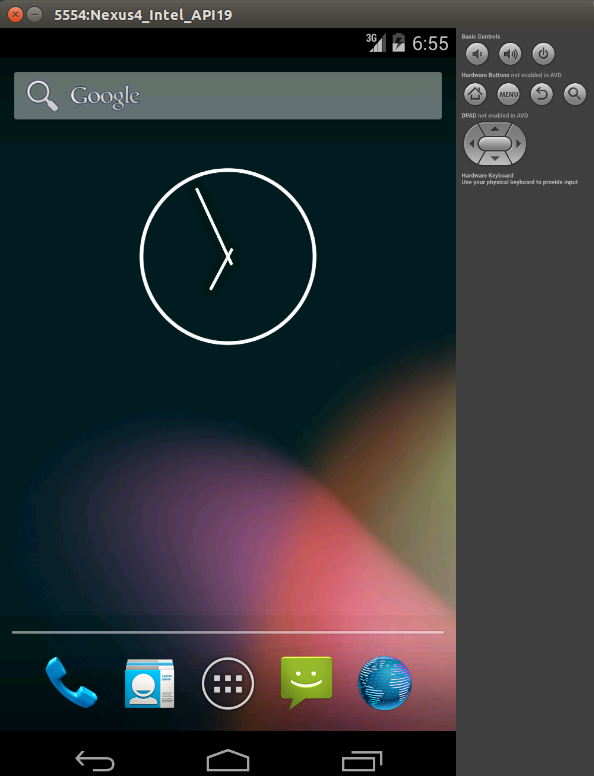
\includegraphics[keepaspectratio, scale=0.3]{Media/Captures/emulator_api_19.png}
      \caption{Emulador Android API 19}
      \label{fig:android_emulator19}
    \end{figure} 
    
    De esta manera podemos probar la aplicación, que será lanzada en el emulador/dispositivo una vez termine su instalación. \\[.2cm]

	\textbf{2 - Teniendo un emulador previamente lanzado (ver sección anterior para ver cómo se lanza) o un dispositivo móvil ya conectado por USB:} \\[.2cm]
	
	En este caso es todavía más sencillo el proceso de construcción. Nos vamos a la carpeta raíz del proyecto  y podemos compilar e instalar la aplicación con un solo comando:

 	 \begin{lstlisting}[style=console, numbers=none]
		$ ant debug install
	\end{lstlisting}	
 	 
 	 Es importante destacar que este comando solo funciona si tenemos un único emulador o dispositivo conectado, de lo contrario habrá que utilizar el método anterior. \\[.2cm]

    
    		\subsubsection{Proceso de Depuración} \label{sssec:debug}
    
    Una vez instalada una aplicación, podemos depurar su código en ejecución usando la herramienta DDMS del ADT en conjunto con la vista de Debug de Eclipse. Pero antes hay que especificar qué aplicación queremos depurar de las que puedan estar instaladas en el dispositivo o emulador. \\[.2cm]

En el caso del emulador debemos lanzar la aplicación llamada “Dev Tools” y abrir el menú “Developer Options”. Dentro de este menú habilitaremos las opciones de “USB debugging” y de  “Wait for debugger”. Además pulsaremos sobre “Select Debug app” y seleccionaremos la aplicación que queremos depurar. \\[.2cm]

En el caso de un dispositivo Android debemos ir a los Ajustes del dispositivo y seleccionar el menú de Opciones de Desarrollador. Aquí habilitamos las opciones de "Depuración de USB"  (si no esta habilitada ya) y de "Esperar al depurador". Además pulsamos donde pone "Seleccione una aplicación para depurar" y elegimos la aplicación que queremos depurar. \\[.2cm]

Una vez hecho esto, cada vez que ejecutemos la aplicacion saldrá un mensaje de advertencia y se quedará esperando a que conectemos un depurador para continuar con su ejecución. Para esto, nos vamos a Eclipse y abrimos la vista de DDMS. Aquí nos aparecerá, entre otras cosas, un espacio con todos los procesos en ejecución en el dispositivo/emulador. Localizamos el proceso de nuestra aplicación y pulsamos sobre el bichillo verde para conectar el depurador a ella. Llegados a este punto la aplicacion continua su ejecución en el emulador y aparece un escarabajo verde al lado del proceso de la app en la ventana de DDMS, que indica que se esta depurando ese proceso. Es entonces cuando podemos abrir la vista de depuración de Eclipse y proceder a trabajar con breakpoints para depurar y estudiar el código con el fin de solucionar errores.

	\subsection{Migración: Identificación y Solución de Problemas}
  
	  El objetivo de esta parte del proyecto es conseguir que el cliente de SwellRT se pueda desplegar en Android para asi conseguir que se conecte al servidor WIAB que tambien incluye. Para ello lo primero que haremos será desplegar el servidor en nuestro ordenador clonando el repositorio de GitHub de SwellRT y siguiendo los pasos descritos en el Readme del proyecto \cite{ref:swellRT_github}. Para comprobar que el servidor se ha instalado correctamente, podemos ejecutarlo por consola (ver Readme) y abrir un navegador web con la dirección http://localhost:9898. Si nos aparece una ventana de Login de WIAB es que ya tenemos un servidor WIAB corriendo en nuestro ordenador. Creamos entonces un usuario y contraseña de prueba. Este paso es importante ya que la aplicación Android intentará conectarse contra este servidor mientras estemos haciendo pruebas de desarrollo. \\[.2cm]
	  
	  A continuación crearemos un proyecto Android en Eclipse e incluiremos en él todas las clases de SwellRT. Uno de los componentes principales de Android a la hora de desarrollar son las \textbf{Actividades} \cite{ref:android_activities}, que representan las pantallas que se le muestran al usuario y que responden a su interacción programáticamente. Por tanto, crearemos una nueva actividad  
	  principal (waveAndroid.java) que se ejecutará al lanzar la aplicación y que por el momento intentará conectarse al servidor especificando por código el usuario y contraseña que hemos creado antes en el servidor. Wave realiza este login contra el servidor usando dos tecnologias: HTTP \cite{ref:http_authentication} y WebSockets \cite{ref:webSocket_ref}.
	  
  
    		\subsubsection{Conexión HTTP}\label{sssec:conHttp}
	
	Wave fue desarrollado para utilizar el protocolo WebSocket para la conexión al servidor, pero esta tecnología necesita realizar una autenticación HTTP previa. Lo primero que haremos será otorgar \textbf{permisos de conexión a internet} a nuestra aplicación. Android utiliza un \textbf{sistema de permisos} \cite{ref:android_permissions} para controlar los privilegios de cada aplicación. Estos permisos se declaran en el \textbf{Manifiesto} de la aplicación \cite{ref:android_manifest}, archivo que declara sus características. Para ello basta con añadir lo siguiente al manifest.xml de la aplicación:
	  
	  \lstset{language=XML, breaklines=true, autogobble=true, basicstyle=\ttfamily\footnotesize}
	  \begin{lstlisting}[frame=single]
	  	<uses-permission android:name="android.permission.INTERNET"/>
	  \end{lstlisting}
	  
	  	 También hay que tener en cuenta que cuando nos encontramos en el emulador no estamos en la misma red que el ordenador en el que trabajamos, por lo que la conexión a la URL http://localhost:9898 no es válida. No obstante, esto tiene facil solución pues \textbf{el emulador de Android define unas direcciones IP de red especiales} \cite{ref:android_netAddress} para este tipo de casos. Basta con sustituir localhost por la direccion 10.0.2.2 para conseguir acceder al servidor WIAB desplegado en el ordenador. La dirección URL sera por tanto: \textbf{http://10.0.2.2:9898}. 
	  
	 Lo siguiente que haremos será ejecutar el código de Login del cliente SwellRT para intentar localizar dónde se lleva a cabo la conexion HTTP. Para ello llamamos desde la actividad principal (WaveAndroid.java) al método startSession() de la clase WaveClient.java pasándole el usuario y la contraseña antes creados.
 
	 Esto provoca un error de ejecución y la aplicación se cierra. Lo siguiente que hacemos es depurar la aplicación (Ver Seccion \ref{sssec:debug}) estudiando el LogCat \cite{ref:android_logcat} (Ver Figura \ref{fig:android_logcat}) para ver dónde se produce el error. Descubrimos que el problema estaba localizado en el método login() de la misma clase, que intentaba realizar una \textbf{petición POST HTTP} al servidor utilizando un \textbf{RequestBuilder} de la librería \textbf{com.google.gwt.http.client}. He aquí el primer problema: la actual conexión utiliza métodos de GWT/Javascript para hacer la petición Post y Android no es compatible con esta tecnología.   
	 
	\begin{figure}[H]
      \centering
	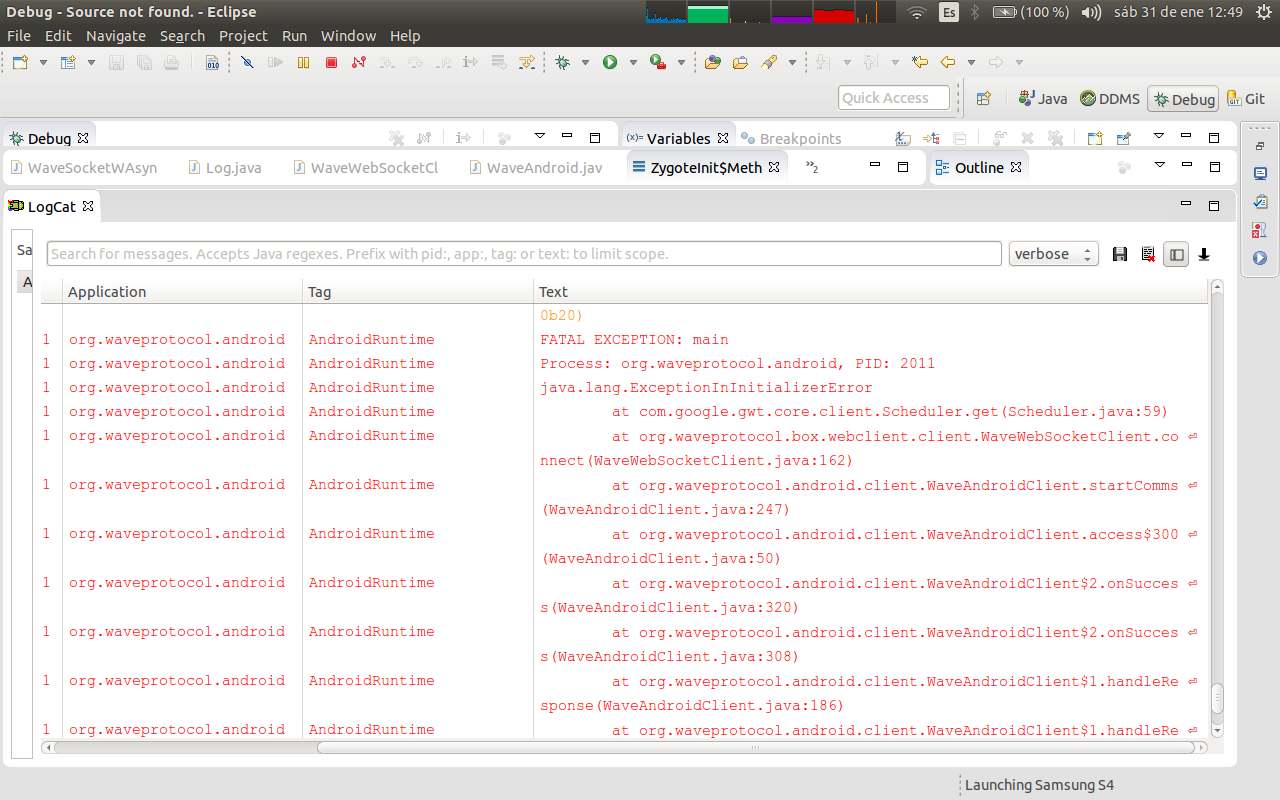
\includegraphics[keepaspectratio, scale=0.3]{Media/Captures/logcat_example.png}
      \caption{Ejemplo de Traza de Error en Logcat}
      \label{fig:android_logcat}
    \end{figure} 
	 
	 Hay por tanto que encontrar una librería similar compatible con Android que construya una petición \textbf{HTTP POST} y la envíe al servidor. La primera opción que valoramos fue utilizar la \textbf{librería HTTP Apache} \cite{ref:apache_http}, incluida en el SDK de Android desde sus primeras versiones. Sin embargo, Google recomienda \cite{ref:http_recommmendations} a partir del API 10 (Android 2.3 "Gingerbread") utilizar la \textbf{librería HttpURLConnection}\cite{ref:android_httpUrlConnection}, también incluida en el API. Por tanto esta última es la que elegimos para la migración. \\[.2cm] 
	 
	 De forma simplificada, éste seria un esquema de la nueva estructura del login HTTP:
	 
	  \lstset{language=Java, breaklines=true, autogobble=true, basicstyle=\ttfamily\footnotesize, commentstyle=\color{OliveGreen}, keywordstyle=\color{MidnightBlue}}
	  \begin{lstlisting}[frame=single]	  
import java.net.HttpURLConnection;

private void login(final String user, final String password, final Callback<String, String> callback) {
  
		//Construct the URL String urlStr with the server, user and password parameters
  
	    URL url = new URL(urlStr); //String 
	    HttpURLConnection connection = (HttpURLConnection) url.openConnection(); //Open the connection to the given URL

	    connection.setDoOutput(true); // allow the POST connection
	    connection.setRequestProperty("Accept-Charset", CHARSET);
	    connection.setRequestProperty("Content-Type", "application/x-www-form-urlencoded;charset="
		+ CHARSET);

	    OutputStream out = connection.getOutputStream(); 
	    out.write(queryStr.getBytes(CHARSET)); //Set the POST parameters

	    if (connection.getResponseCode() != 200) {
		      //ERROR during the connection
		      connection.disconnect(); //Disconnect from the server.
	    } else {
		      //Continue with the login process (WebSocket)
		      connection.disconnect(); //Disconnect from the server.
	    }		      
}	    
	  \end{lstlisting}  
	  
	  Sin embargo, aquí no acaba el problema. Por cuestiones de usabilidad y de respuesta a la interacción del usuario, Android establece dos reglas para trabajar con el proceso de la actividad que se le esta mostrando al usuario (llamado \textbf{UI Thread}) \cite{ref:android_processes}:
	  
	  \begin{itemize}
	  	\item \textbf{1. No bloquear el UI Thread}
	  	\item \textbf{2. No acceder al UI Thread directamente desde otro Thread}
	  \end{itemize}
	  
	  La conexión a un servidor es un proceso susceptible de durar un tiempo variable según las condiciones de la red, lo cual deja la aplicación en espera hasta que se realiza dicha conexión,  bloqueando el UI Thread. Por tanto, decidimos usar un hilo (Thread) por separado en forma de \textbf{AsyncTask} \cite{ref:android:asynctask} para llevar a cabo la tarea de Login, tal y como recomienda Google hacer para trabajar con conexiones a la red \cite{ref:android_networking}. La ventaja por tanto de usar otro hilo para esto es que la actividad principal no se bloquea. \\[.2cm]
	  	 
	 Es importante también destacar que la arquitectura de SwellRT y de Wave está planteada de manera que utiliza llamadas asíncronas (callbacks) para notificar al resto de la aplicacion del resultado de los procesos de conexión al servidor, por lo que nuestro AsyncTask tendrá que usar el callback apropiado para notificar del éxito o fracaso de la conexión Http.
	 
	  El siguiente es un esquema del AsyncTask encargado del Login: \\[.2cm]
	  
	  \lstset{language=Java, breaklines=true, autogobble=true, basicstyle=\ttfamily\footnotesize, commentstyle=\color{OliveGreen}, keywordstyle=\color{MidnightBlue}}
	  \begin{lstlisting}[frame=single]	  
private class LoginTask extends AsyncTask<String, Void, String> {
    @Override
    protected String doInBackground(String... params) { //method that executes on the new Thread without blocking the UI Thread
      login(params[0], params[1], params[2]); //Do the login 
      return sessionId //String needed for the WebSocket connection and based on the cookie received from the server.     
    }
    @Override
    protected void onPostExecute(String result) { //method that executes on the UI Thread once doInBackground() finishes its execution.    
      if (result != null) { 
        callback.onLogin(); //Notify the login success using the proper callback method
      } else { //The doInBackGround method has had a problem and the result of its execution was null
        callback.onError("Wave Login Error"); //Notify the login error using the proper callback method
      }
    }
}    
	  \end{lstlisting} 
	  
	  Este proceso de conexión Http nos deberá devolver una Cookie que trataremos con el onjetivo de generar un SessionId que será necesario para seguir con la conexión al servidor. \textbf{Llegados a este punto, tenemos un proceso de login Http que hace uso de la librería HttpUrlConnection y de un AsyncTask para realizar esa primera conexión al servidor.} Depuramos la aplicación y comprobamos que efectivamente el login Http se realiza correctamente (la respuesta del servidor tiene código 200). \textbf{Sin embargo la aplicación aún no funciona correctamente, pues se cierra al intentar ejecutar el código que se encarga del siguiente paso de la conexión: conectarse por WebSocket.}    
    
    		\subsubsection{Conexión WebSocket}\label{sssec:conWave}
    
    Para realizar una conexión con el servidor Wave es necesaria una conexión mediante WebSockets\cite{ref:webSocket_ref}, tecnología que permite conexiones bidireccionales y asíncronas entre el servidor y el cliente (recordemos que la conexión en el modelo cliente-servidor tradicional está definida como unidireccional de cliente a servidor), de manera que cualquiera de los dos puede iniciar una conexión con el otro en cualquier momento e intercambiar información con éste. En el caso del protocolo Wave este comportamiento es el deseable, ya que al tratarse de un protocolo de comunicaciones federado en el que cualquiera en la red puede ser cliente o servidor, es importante que la conexión sea bidireccional. Además la asincronía es necesaria ya que para mantener la consistencia en tiempo real \ref{sssec:realTime} hace falta que el servidor que contiene las waves pueda iniciar una conexión con los clientes para notificar los cambios que se produzcan en dichas waves. Por tanto, nuestro cliente Android debe ahora establecer una conexión WebSocket con el servidor WIAB. 
    
    La metodología a utilizar será la misma que para la conexión HTTP, se ejecutará el código de SwellRT para identificar dónde falla y por tanto cómo está estructurada la creación y gestión de WebSockets en la versión GWT.
    
    El cliente SwellRT original realiza esta conexión utilizando una librería llamada Atmosphere \cite{ref:atmosphere}, que proporciona un framework para Java que permite gestionar conexiones WebSocket junto a la conexión HTTP que subyace por debajo. Sin embargo, esta librería se encarga solo de gestionar la conexión, no de crear el WebSocket propiamente dicho. En el caso de SwellRT este WebSocket se crea utilizando la implementación que proporciona GWT llamada también WebSocket (WebSocket.java). Esta clase nos define las funciones básicas que debería tener nuestro WebSocket: \textbf{onOpen()} para establecer la conexión, \textbf{onMessage()} para recibir mensajes por el WebSocket, \textbf{send()} para enviar mensajes y \textbf{onClose()} para cerrar la conexión. Asímismo nuestro Websocket deberá también implementar una serie de callbacks (definidos en la interfaz WebSocketCallback.java) para notificar a la aplicación de la llegada de estos eventos del servidor. Los callbacks son: \textbf{onConnect()}, \textbf{onDisconnect()} y \textbf{onMessage(message)} respectivamente.
	
	Este WebSocket se crea utilizando un \textbf{patrón de diseño Factory}, que abstrae la creación de un objeto de su implementación, de manera que el desarrollador tenga acceso al objeto sin tener que preocuparse de cómo este implementado el WebSocket por debajo (ver WaveSocketFactory.java en SwellRT). En este caso, como ya se ha dicho, con Atmosphere y WebSocket GWT. No obstante, la aplicación no funciona tal y como está hecho en SwellRT ya que android no soporta GWT de forma nativa. Hay que sustituir este código buscando una librería open-source que implemente un WebSocket en Android sobre Atmosphere y que porporcione las mismas funciones básicas descritas en el párrafo anterior.
	
	La solución encontrada fue utilizar wAsync\cite{ref:wAsync_github}, librería proporcionada por Atmosphere para trabajar con Websockets en Node.js, Java y Android. wAsync trabaja creando un socket que responde a eventos diversos, estando entre ellos eventos similares a los utilizados por la versión GWT de SwellRT: \textbf{on(EVENT.name())}, siendo EVENT el nombre del evento al que debe responder. Un ejemplo sencillo de utilización de wAsync sería el siguiente:
	
	\lstset{language=Java, breaklines=true, autogobble=true, basicstyle=\ttfamily\footnotesize, commentstyle=\color{OliveGreen}, keywordstyle=\color{MidnightBlue}}
	  \begin{lstlisting}[frame=single]	  	  
	  //Create the atmosphere client
	  AtmosphereClient client = ClientFactory.getDefault().newClient(AtmosphereClient.class);
	  //Configure client with URL
      AtmosphereRequestBuilder requestBuilder = client.newRequestBuilder()
          .method(Request.METHOD.GET).trackMessageLength(true).uri(WaveSocketWAsync.this.urlBase)
          .transport(Request.TRANSPORT.WEBSOCKET)
	 //Create and configure socket
      WaveSocketWAsync.this.socket = client.create(client.newOptionsBuilder().runtime(ahc).build())
          .on(Event.OPEN.name(), new Function<String>() { //Equivalent to GWT onOpen() method
            @Override
            public void on(String arg0) {
			// set the actions to do and call the proper callback function (callback.onConnect())
            }
          }).on(Event.CLOSE.name(), new Function<String>() { //Equivalent to GWT onClose() method
            @Override
            public void on(String arg0) {
            // set the actions to do and call the proper callback function (callback.onDisconnect())
            }
          }).on(Event.MESSAGE.name(), new Function<String>() {
            @Override
            public void on(String arg) { //Equivalent to GWT onMessage() method
            // set the actions to do and call the proper callback function (callback.onMessage())
            }
          }).on(new Function<Throwable>() {
            @Override
            public void on(Throwable t) {
   			// catch possible exceptions
            }
          });
      try {
      	// connect to the server
        socket.open(requestBuilder.build());
      } catch (IOException e) {
		// catch possible exceptions
      } 
      //send a given message to the server, equivalent to GWT send(msg) method 
      socket.fire(Data);
	\end{lstlisting}
	
	Como la arquitectura Wave utilizaba el patrón factoria, fue necesario sustituir la clase de WebSocket GWT por una de nueva creación llamada \textbf{WaveSocketWAsync.java}\cite{ref:wave_migration_github} que implementa los métodos de creación y configuración de un Websocket y de callback antes descritos. Asimismo se modificó la clase WaveSocketFactory.java para hacer uso ahora de esta nueva implementación del WebSocket compatible con Android. 
	
	Sin embargo, ejecutamos esta nueva versión de código y nos encontramos con que la librería WAsync incluye dependencias a código que no está presente en la propia librería y que es necesario para crear el cliente AsyncHTTPClient que gestiona la conexión HTTP que subyace por debajo del WebSocket. Concretamente hace falta utilizar un HTTPProvider compatible con Atmosphere, tal y como recomienda hacer wAsync en su wiki\ref{cite:httpProvider_wAsync}. Para ello basta con añadir al proyecto las librerias oportunas (Ver Tabla de dependencias \ref{fig:dependencies_swellRT}) y configurar el cliente segun lo descrito en dicha wiki:
		
	\lstset{language=Java, breaklines=true, autogobble=true, basicstyle=\ttfamily\footnotesize, commentstyle=\color{OliveGreen}, keywordstyle=\color{MidnightBlue}}
	  \begin{lstlisting}[frame=single]	
	  AsyncHttpClientConfig ahcConfig = new AsyncHttpClientConfig.Builder().build();
      AsyncHttpClient ahc = new AsyncHttpClient(new GrizzlyAsyncHttpProvider(ahcConfig));
      \end{lstlisting}
      
      Ahora, al ejecutar la aplicación comprobamos que la conexión al servidor se produce correctamente. Para completar esta parte del proyecto solo falta pedir al usuario su user y password, ya que hasta ahora las habiamos especificado a mano en el propio código para realizar pruebas.
	    
    		\subsubsection{Conexión final y Logging}
    
    Para probar que la aplicación migrada es funcional y es capaz de utilizar las características nativas de Android haremos una pequeña y sencilla pantalla de Login que pedirá al usuario la dirección del servidor Wave, un usuario y una contraseña.
    
    En el diseño de aplicaciones Android el componente principal de una app es la Actividad, que se corresponde con la pantalla con la que interactúa el usuario. La interfaz gráfica se usuario (UI) de las pantallas se encuentra separada del código de la aplicación en ficheros xml de Layout\cite{ref:android_ui}. A una Actividad se le especifica cuál es su archivo de layout en su método onCreate(), responsable de la creación de la actividad y sus recursos. 
    
    Creamos una Actividad llamada WaveAndroid.java que haga uso del layout Main.xml, en el cual incluimos tres cajas de texto (llamadas EditText en Android) para que el usuario introduzca los datos. Además guardamos una referencia a estas cajas de texto en la Actividad para poder acceder al texto introducido y pasárselo al método login de Wave que hemos migrado anteriormente.
    
    	\begin{figure}[H]
      \centering
	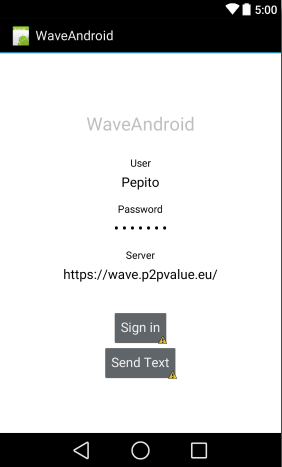
\includegraphics[keepaspectratio, scale=0.6]{Media/Captures/waveAndroidLogin.png}
      \caption{Pantalla de Login de WaveAndroid}
      \label{fig:android_waveLogin}
    \end{figure}
    
    Además decidimos mejorar el sistema de mensajes de Log de la aplicación sustituyendo el framework de la librería SLF4J para Java usada por SwellRT por una versión más reciente desarrollada para Android\cite{ref:slf4j_android}.
        
    Por último instalamos la aplicación en el emulador o el dispositivo móvil y probamos que se nos muestra la pantalla de login anterior. Introducimos los datos del servidor WIAB (en este caso utilizaremos el servidor de P2PValue desplegado para pruebas en https://wave.p2pvalue.eu/), de usuario, contraseña y comprobamos que hemos conseguido el objetivo de esta parte del proyecto: \textbf{nuestro cliente Android realiza el login contra el servidor WIAB correctamente.} 
     
    		\subsubsection{Organización del código: Servicio Android}
    
    Una vez conseguida la conexión al servidor desde Android, decidimos revisar el código para intentar optimizarlo y organizarlo de manera que aprovechara mejor las características de Android y la arquitectura de Wave. Además, el API que permite gestionar el modelo de datos de SwellRT (Ver Sección \ref{sssec:swellRT}) está escrito en java, por lo que es plenamente funcional y compatible con el código de nuestra migración a Android. A continuación hablaremos de los motivos de dicha reorganización.
  
    Como ya se ha comentado anteriormente, el proceso de login se debe hacer en un hilo de ejecución separado del hilo principal o UI Thread, ya que Android no recomienda\cite{ref:android_processes} que tareas que tarden mucho tiempo en ejecutarse (cómo por ejemplo descarga de datos de la red) se ejecuten en el mismo hilo que la interfaz de usuario, pudiendo bloquear dicho hilo y obstaculizando por tanto la interacción del usuario con el dispositivo.
      
    Hasta ahora habíamos utilizado para ello una Actividad que cotenía el AsyncTask \cite{ref:android_asynctask} encargado de ejecutar el código de conexión al servidor en un hilo separado del UI Thread. Sin embargo, tal y como está definida la arquitectura de Wave y de SwellRT, la utilización de callbacks (ver secciones \ref{sssec:conHttp} y \ref{sssec:conWave}) es necesaria para notificar al resto de la aplicación de los eventos relacionados con el intercambio de datos con el servidor. Un AsyncTask ejecuta de una sola vez y de forma asíncrona el código que se le asigne a su método doInBackground(), de manera que una vez que termina su ejecución puede notificar el resultado de la conexión, pero no queda a la espera de otros posibles eventos en el socket (como la recepción de mensajes o la desconexión). Es decir: \textbf{aunque se definan callbacks para esperar los eventos del servidor, el socket no podrá notificarlo porque no existe un hilo que quede a la espera de estos eventos.}

    Por otro lado, cada vez que quisiéramos realizar algún tipo de interacción con el servidor habría que utilizar un AsyncTask específico para ello, lo cual no hace sino añadir más código a la aplicación. Otra desventaja de los AsyncTask en la implementación inicial es que si la Actividad que lo esta ejecutando pasa a segundo plano (por ejemplo si el usuario cambia de aplicación) se detiene el proceso de conexión. 

    Considerando todo esto decidimos utilizar otro componente de Android pensado para ejecutar tareas en background y con la opción de hacerlo de forma independiente de la aplicación: el Servicio\cite{ref:android_service}.

    Un Servicio Android se diferencia de una Actividad en que es un componente que se ejecuta en segundo plano y no proporciona una interfaz de usuario con la que éste pueda interactuar. Un Servicio ejecuta tareas de larga duración (cómo la descarga de datos de la red) a petición de otros componentes de la aplicación que estén \textit{suscritos} (el término utilizado por android es \textit{bind}) a dicho Servicio, a modo de cliente-servidor. De esta manera la Actividad (cliente) que se suscriba al Servicio (servidor) puede interactuar con éste último haciendo peticiones y recibiendo notificaciones cuando el Servicio obtenga resultados. \textbf{Por tanto, podremos acceder a la conexión al servidor desde cualquier punto de la aplicación, solo es necesario que la Actividad en ejecución se suscriba al Servicio para hacerlo}. 
    
    Pero un Servicio se ejecuta dentro del mismo proceso que el UI Thread, por lo que aun así tendremos que utilizar métodos para ejecutar el código que nos interese en otros hilos de ejecución dentro del propio Servicio. De esta manera \textbf{se dividió la reorganización en dos: la conexión Http y la conexión WebSocket.}
    
    Para la conexión HTTP, se decidió utilizar un AsyncTask llamado LoginTask muy similar al ya explicado anteriormente (ver Sección \ref{sssec:conHttp}) pero esta vez definido dentro del propio Servicio y con un callback que notificaba a la aplicación si la conexión se realizaba correctamente. Además, se puso el código de la conexión en una clase aparte llamada WaveHttpLogin.java para tenerlo más organizado. El siguiente es un esquema en forma de Diagrama de Secuencia de la conexión Http:
    
  \begin{figure}[H]
   \centering
	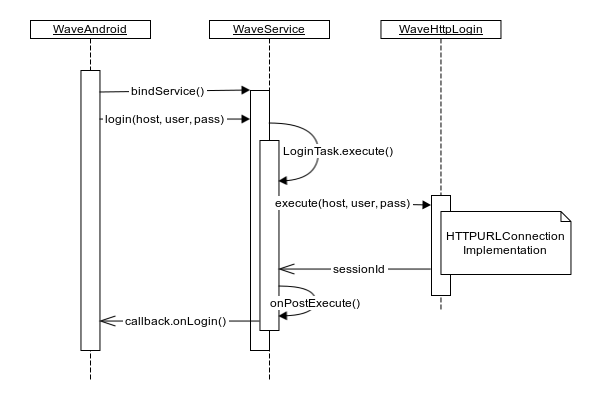
\includegraphics[keepaspectratio, scale=0.6]{Media/Diagrams/loginHttpSequenceDiagram.png}
    \caption{Proceso de conexión Http con Servicio}
   \label{fig:sequenceDiagram_waveHttp}
  \end{figure}
    
    Como vemos, cuando se realiza esta conexión Http la Actividad inicial (WaveAndroid.java) es informada de ello mediante su callback onLogin() para poder notificar al usuario e iniciar la conexión por WebSocket. 
    
    Para dicha conexión se debía buscar una solución que permitiera al WebSocket responder a eventos del servidor (recordemos el funcionamiento de WAsync descrito en la Sección \ref{sssec:conWave}) para, mediante callbacks, informar a la aplicación de dichos eventos. \textbf{La solución final encontrada fue combinar el uso de un Thread y un Handler}. El Thread se encarga de crear el socket y configurar su respuesta a eventos en forma de mensajes, que enviará entonces al Handler, encargado de quedar a la espera de recibir estos mensajes de forma asíncrona y llamar al callback adecuado. Esta imnplementación se puede ver concretamente dentro de la clase WaveSocketWAsync.java, donde se define el Thread llamado WebSocketRunnable y el Handler UIHandler. El siguiente es un esquema en forma de Diagrama de Secuencia de la conexión inicial con WebSocket al servidor Wave:
    
  \begin{figure}[H]
   \centering
	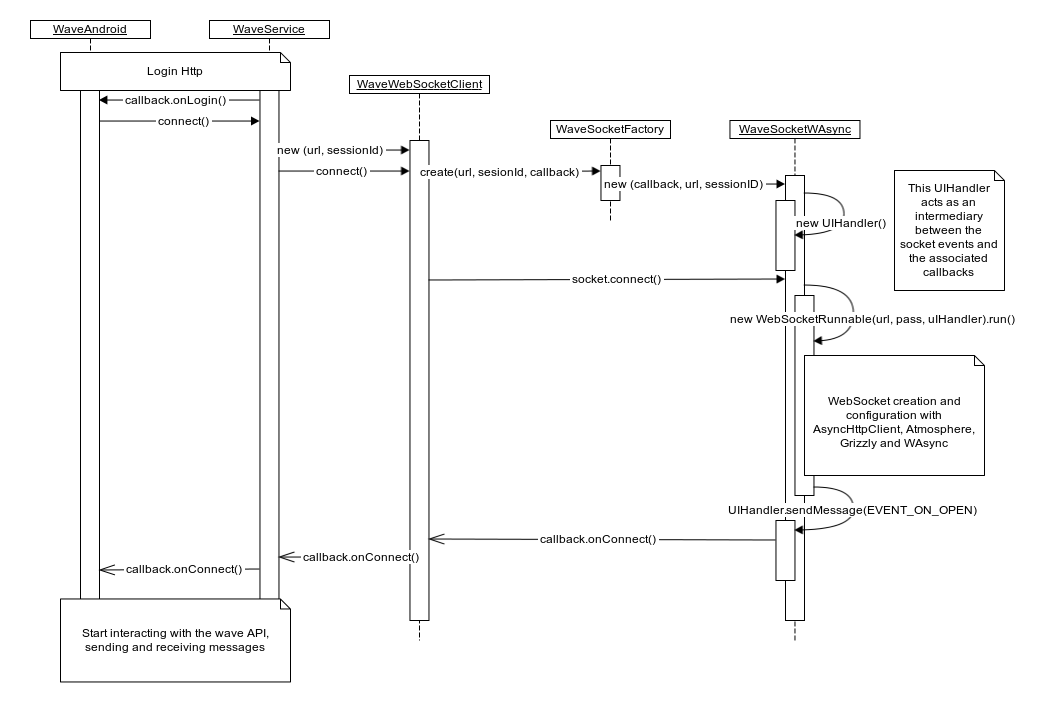
\includegraphics[keepaspectratio, scale=0.43]{Media/Diagrams/waveServerConnectionSequenceDiagram.png}
    \caption{Proceso de conexión WebSocket con Servicio}
   \label{fig:sequenceDiagram_waveWebSocket}
  \end{figure}
     
      Como vemos, cuando se realiza esta conexión al Servidor Wave la Actividad es notificada de ello mediante la propagación de callbacks onConnect() que informan del éxito de la conexión. A partir de este momento el socket informará de la misma forma (mediante el envío de mensajes al UIHandler) de otros eventos que se produzcan, ya sea la recepción de datos o la desconexión por ejemplo. De la misma forma la aplicación podrá enviar datos al servidor, ya que el socket se mantiene en el Servicio. 
       
    \subsection{Dependencias}
    
    El cliente Android de SwellRT migrado y desarrollado en esta parte del proyecto hace uso de las siguientes dependencias con librerías externas a Android:

    \begin{table}[h]
      \footnotesize
      \begin{center}
	\begin{tabular}{ | c | c | m{8cm} | }
	  \hline
	  \textbf{Nombre} & \textbf{Versión} & \textbf{Descripción} \\
	  \hline
	  WAsync \cite{ref:wAsync_github} & 1.4.3 & WebSockets/HTTP Client Library for Asynchronous Communication \\ 
	  \hline
	  AsyncHttpClient \cite{ref:asyncHttpClient} & 1.8.14 & Library that allows Java applications to easily execute HTTP requests and asynchronously process the HTTP responses.\\ 
	  \hline
	  Grizzly-Framework \cite{ref:grizzly} & \multirow{3}{*}{2.3.18} & Core framework for Grizzly applications that provides TCP/UDP transports, memory management services/buffers, NIO event loop/filter chains/filters. \\ \cline{1-1} \cline{3-3} 
	  Grizzly-Http \cite{ref:grizzly} & & HTTP framework that contains the base logic for dealing with HTTP messages on both the server and client sides. \\ 
	  \cline{1-1} \cline{3-3} 
	  Grizzly-WebSockets \cite{ref:grizzly} & & WebSockets custom API for building Websocket applications on both the server and client sides. \\ 
	  \hline
	  slf4j-Android \cite{ref:slf4j_android} & 1.6.1 & Simple Logging Facade for Java: logging framework for Android \\ 
	  \hline
	\end{tabular}
      \end{center}
      \caption{Dependencias de SwellRT-Android}
      \label{fig:dependencies_swellRT}
    \end{table}       
       
    \subsection{Resultado de la Migración}
    
    Después de todos estos pasos disponíamos de una versión funcional de SwellRT capaz de conectarse al servidor WIAB de forma nativa desde Android. \textbf{El resultado de esto se puede ver en el GitHub de esta parte del proyecto}\cite{ref:wave_migration_github}. El siguiente es un esquema en forma de Diagrama de Clases del resultado final:
    
  \begin{figure}[H]
   \centering
	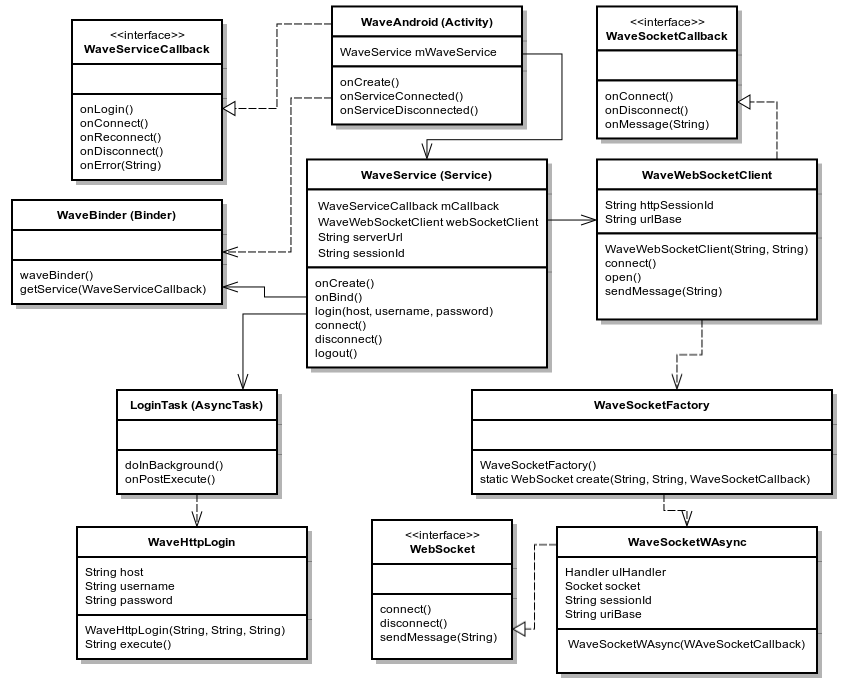
\includegraphics[keepaspectratio, scale=0.5]{Media/Diagrams/waveServiceClassDiagram.png}
    \caption{Esquema de Clases de SwellRT-Android con Servicio}
   \label{fig:sequenceDiagram_waveWebSocket}
  \end{figure}
    
    Solo restaba poner el API de SwellRT encima de lo nuestro para poder acceder y trabajar a nivel de wave con el modelo de datos de SwellRT. De esto se encargó uno de los desarrolladores del proyecto inicial, Pablo Ojanguren, con el cual habiamos trabajado para realizar lo anteriormente descrito.
    
    El API con el cliente de SwellRT adaptado a Android, con el cual trabajaremos en la siguiente parte del proyecto para crear una aplicación Android que haga uso de ello, se encuentra en el GitHub de SwellRT\cite{ref:swellRT_android_github}. 


\section{Diseño de la Aplicación: Diseño Guiado Por Objetivos}

Para elaborar el diseño de la aplicación, nos hemos basado en la metodología del Diseño Guiado por Objetivos, que implementa el proceso de la Ingeniería de la Usabilidad propuesto por Alan Cooper \cite{ref:bookAlanCooper}. Este proceso constará de las siguientes fases:

EXPLICARLOS: TEMA 3 PAGINA 21 DSI

\begin{itemize}
	\item \textbf{1. Investigación}
	\item \textbf{2. Modelado}
	\item \textbf{3. Definición de Requisitos}
	\item \textbf{4. Framework de Diseño}
\end{itemize}

Queremos insistir eso sí en que únicamente nos hemos basado en esta metodología para seguir el proceso del diseño de la aplicación. No seguiremos todas las fases de esta metodología al pie de la letra ya que el alcance en tiempo de este proyecto escapa a una metodología tan formal y laboriosa (que implica gran cantidad de pruebas y procesos) como esta.

\subsection{Investigación}

\subsubsection{Intención Inicial: Prototipo básico}  

¿HABLAR DE INTENCION FUTURA PARA ELECCIONES?


\underline{Programas electorales}

La intención fundamental de la aplicación es llevar los programas electorales a los bolsillos de los ciudadanos y generar interés en participar más activamente en la política, ya sea emitiendo opiniones sobre dichos programas o elaborando nuevas propuestas. Vivimos en una sociedad digital, donde cada vez son más las personas que utilizan sus smartphones para realizar todo tipo de tareas en su vida cotidiana.

En los últimos años las diferentes formaciones políticas han subido sus programas electorales a un documento en formato PDF que suele estar disponible para su descarga en su página web. Este documento tiene generalmente una gran extensión (los hay de 200 páginas), lo cual no hace sino dificultar que las personas se animen a leerlo. Por ello pensamos que una aplicación que pudiera visualizar las principales secciones de los programas políticos podría ser especialmente útil para acercar los programas a los electores.

Además también intentariamos darle una estructura a estos programas, de manera que el usuario pudiera navegar por ellos a nivel de Sección, a diferencia del método actual de leer un "macro-documento" en PDF. Así, la gente podría opinar sobre los programas políticos a nivel de sección mediante acciones familiares para ellos: "Me gusta", "No me gusta" y realizar "Comentarios". Añadimos también una acción de "No lo entiendo" que pensamos que seria util para indicar cuándo la redacción de la sección era de significado difuso.

En definitiva, queríamos crear un espacio donde poder informarse sobre las distintas ofertas electorales y poder debatir sobre las propuestas que propone cada formación política, todo ello en forma una aplicación que podremos consultar en cualquier momento. 

\underline{Propuestas y Wave}

Por otro lado,y en línea con los últimos movimientos políticos ciudadanos, pretendíamos crear también un portal de propuestas ciudadanas en el móvil. Los usuarios podrían visualizar las propuestas de otros usuarios y tener la posibilidad de crear nuevas propuestas. Además, como queríamos aprovechar las características de la migración de Wave previamente desarrollada, pensamos en la posibilidad de elaborar estas propuestas de forma colaborativa y en tiempo real entre muchos usuarios.

Actualmente existen multitud de portales (en su gran mayoría web) donde la ciudadanía puede expresar su opinión, pero creemos que la integración de una aplicación donde puedan situarse las opiniones de los partidos políticos (en forma de sus programas) y la actividad ciudadana (en forma de propuestas), genera una nueva manera de tratar la política en los medios sociales.

También pensamos en la posibilidad de categorizar el contenido de la aplicación (Programas y Propuestas) por temas, para proporcionar filtros a la hora de navegar por dicho contenido. Sin embargo no teníamos muy clara la elección de temas, asi como si debiamos darle al usuario la posibilidad de crear nuevos temas o dar nosotros unos temas preestablecidos.
 
Una vez pensada la intención y los principales objetivos de la aplicación, procedimos a realizar unos primeros prototipos en papel de nuestra idea y a implementar un prototipo básico en el móvil (Ver Sección \ref{ssec:prototypes}) que mostraba programas políticos estructurados y permitía navegar a nivel de Sección por ellos para leer y emitir opiniones (likes, dislikes, comentarios, etc.).  

HIPOTESIS DE PERSONAS pag 24

 El siguiente paso sería estudiar la viabilidad de esta aplicación entrevistando gente para realizar una investigación sobre sus necesidades prácticas. Por otra parte también sería útil enseñarles los prototipos básicos que manejábamos para verificarlos. Entendimos que el tipo de persona con el que nos entrevistáramos debía de estar relacionado de alguna manera con el mundo de la política, pues nada mejor que hablar con gente ya interesada en dichos temas para orientarnos por el buen camino.

A continuación detallamos las entrevistas que realizamos en la investigación:

\subsubsection{Entrevista con Labodemo}

Tuvimos la oportunidad de mantener una conversación con dos miembros de Labodemo \cite{ref:labodemo}, en la que aprovechamos para mostrarles un prototipo de la aplicación que estábamos desarrollando. Ambos tenían experiencia en el desarrollo de plataformas de participación ciudadana en Internet: fueron los responsables del desarrollo de los portales de participación del partido político Podemos y la candidatura ciudadana de unidad popular Ahora Madrid.

En ese momento nuestro prototipo móvil se limitaba únicamente a mostrar las diferentes secciones de cada programa, lo cual les pareció útil, aunque no lo suficiente como para atraer a una cantidad considerable de usuarios. Conforme a su linea de trabajo habitual, eran más partidarios de dar a los usuarios la posibilidad de realizar Propuestas además de ver Programas políticos. Les comentamos entonces que antes de hablar con ellos ya habíamos planteado desarrollar Propuestas colaborativas en tiempo real aprovechando la tecnología de Wave. Pero ellos no eran partidarios de esta opción, ya que según ellos acabaría siendo caótico tener tanta gente editando la misma propuesta de cara a generar contenido útil. 

Dándole una vuelta a la categorización del contenido, nos sugirieron que para atraer a usuarios, debíamos considerar la posibilidad de integrar en la aplicación a colectivos sociales que generaran y categorizaran dicho contenido. No eran partidarios de que dieramos nosotros ciertas temáticas preestablecidas, pues debido a la variedad de redaccion en los distintos programas sería dificil identificar temáticas que incluyeran a todos los programas y probablemente acabariamos excluyendo temas. Así, serían los colectivos los que se encargaran de "tematizar" el contenido de la aplicación. Por ejemplo: un grupo de animalistas podría tener un espacio en la aplicación donde poder crear sus propias propuestas, e incluso hacer comparativas de lo que proponen los diferentes programas sobre los animales. 

De esta manera, y en relación a la aproximación a los foros tradicionales, se planteó la idea de crear "Hilos": elementos "temáticos" que agruparan en un solo sitio Secciones y Propuestas que hablaran sobre un determinado tema. Estos hilos serían también generados por dichos colectivos.

Esto sería útil también para usuarios que buscaran información sobre un determinado tema. Por ejemplo: un usuario poco activo, que resulta ser profesor, podría buscar un colectivo de profesores y ver las Propuestas que se llevan a cabo o visualizar una comparativa respecto las medidas de educación de los diferentes programas políticos.

Nos insistieron mucho en el tema de las comparativas. Sería de gran utilidad que la aplicación tuviera una parte de comparativas en la que los usuarios pudieran comparar los programas políticos en vez de leerlos sección por sección. Resultaría de gran interés a un autónomo visualizar las medidas que proponen los diferentes partidos políticos para los autónomos. Pero estas comparativas no podría realizarlas cualquiera, por lo que deberían realizarlas periodistas o expertos que hubieran realizado algún tipo de comparativa similar anteriormente. Nos sugirieron contactar con periodistas o colectivos que hubieran publicado algún tipo de comparativa en cuanto a programas o medidas, para obtener algún tipo de ayuda o consejo a seguir.

\subsubsection{Conclusión}

¿QUE OPINAN Y COMO CAMBIAN LOS PROTOTIPOS? 

La reunión con dos de los miembros de Labodemo resultó de gran interés. Se trataba de personas que tenían mucha experiencia en desarrollo de portales de participación ciudadana y que sobre todo estaban muy familiarizados con el uso común que le suele dar la gente a este tipo de aplicaciones. A priori, sabían mejor que nosotros cómo determinar las claves para que una aplicación tuviera una aceptación y uso considerable de los usuarios desde el principio.

Visualizar los programas políticos en la app no les entusiasmó demasiado. Expusieron que, a priori, un ciudadano de a pie no iba a molestarse en meterse en la aplicación para leer los programas políticos de los diversos partidos. Ellos argumentaban que los colectivos sociales serían los usuarios más activos en nuestra aplicación, por lo que debíamos enfocar más el desarrollo hacia la participación ciudadana y la generación de Propuestas o Comparativas de Secciones de Programas hechas por tales colectivos. Dichas Comparativas sí que generarían más interés por leer los programas políticos.

Tras la reunión tomamos nota de los consejos que obtuvimos de Labodemo. Incluimos la idea de "Comparativas" y empezamos a pensar la forma de colaborar de grupos y colectivos. También intentamos contactar con colectivos y personas interesadas en el desarrollo de la aplicación. 

Finalmente, conseguimos concretar una entrevista con Javier de la Cueva \cite{ref:jdelacueva}.

\subsubsection{Entrevista con Javier de la Cueva}

La entrevista con Javier de la Cueva resultó bastante productiva. Ya le conocíamos de algunas conferencias que impartió en la facultad. Javier es abogado y doctorado en Filosofía, estando especializado en temas relacionados con tecnología, Internet y propiedad intelectual. Además, en sus últimas conferencias Javier habla sobre acciones micropolíticas \cite{ref:manualCiberactivista}. Estas acciones definen la capacidad que tienen los ciudadanos para realizar aportaciones a la sociedad, el estado o el gobierno que favorezcan la participación ciudadana en una democracia participativa.

Representar los programas electorales en una aplicación móvil le pareció algo interesante y necesario para la sociedad actual. Si bien casi nadie hace el esfuerzo de visualizar un programa electoral en PDF, utilizar una herramienta que facilita el acceso al programa por secciones podría ser una nueva forma de incentivar su lectura y ayudar a fomentar la participación ciudadana en política. 

Además nos sugirió la posibilidad de desarrollar una Hemeroteca de programas electorales. De esta forma cualquiera podría consultar los programas de los anteriores gobiernos y comprobar si se cumplieron los objetivos del programa, así como comparar programas de distintos años entre sí, 

Pero si en algo nos insistió Javier, fue en la importancia de categorizar el contenido de la aplicación. Un usuario que no tenga conocimientos sobre diversos temas, se encontraría más cómodo si pudiera visualizar las diferentes partes de un programa o las propuestas ciudadanas por categorías o temas generales. Ya que dejar libertad a los usuarios para crear categorías personalizadas podría ser algo negativo para usuarios inexpertos o con pocos conocimientos sobre temas específicos.

Por último, centrándonos en las Propuestas ciudadanas, surgió la idea de elaborar propuestas que tuvieran una especificación concreta. Es decir, a parte de tener una idea de propuesta y redactarla, esta propuesta debería ir acompañada de los recursos que serían necesarios y sobre todo cómo se llevaría a cabo de una forma aproximada. También resultaría interesante definir un pequeño presupuesto de lo que conllevaría realizar la propuesta o cómo se podría financiar. Así evitaríamos una elaboración de propuestas más real, evitando un listado de propuestas infinito sin planterase cómo se llevarían a cabo o cómo se financiarían.

\subsubsection{Conclusión}

¿QUE OPINAN Y COMO CAMBIAN LOS PROTOTIPOS? 

Javier trató de abrirnos un poco más la mente, para plantearnos ideas que no están representadas en la sociedad. En la actualidad encontramos diversas plataformas de participación ciudadana que acaban convirtiéndose en un foro. Para evitar caer en esto, debíamos innovar algo más para volver a repetir esto, debíamos de intentar desarrollar nuevas formas de participación.

Clasificar nosotros las secciones de un programa así como también las propuestas ciudadanas en diferentes categorías y temas era algo que descartamos en un principio tras la reunión con Labodemo. Aunque para dar cierta libertad, podríamos incluir la posibilidad de crear categorías personalizadas o ir añadiendo categorías semanalmente.

\subsection{Modelado de Personas}

¿QUE SON LAS PERSONAS? -> REPRESENTACION GRAFICA

En esta fase definiremos el tipo de persona que interactuará con nuestra aplicación. Para ello hemos identificado dos tipos de personas primarias:

\textbf{- Activista social, 16 años en adelante}

\underline{Actividad:}

\begin{itemize}
\item Estudia, trabaja o realiza otras actividades de voluntariado.
\item Frecuenta asambleas, participa en diferentes movimientos sociales y está al día de la actualidad política.
\item Utiliza redes sociales para comunicarse con otros colectivos, acudir a asambleas, promover ideas u otras actividades relacionadas con la política y el activismo social.
\end{itemize}

\underline{Otros:}

\begin{itemize}
\item Desconoce las ideas que proponen algunos partidos 
\item Le gusta aportar nuevas soluciones a la sociedad.
\end{itemize}

\textbf{- Ciudadano de a pie, 18 años en adelante}

\underline{Actividad:}

\begin{itemize}
\item Estudia, trabaja o realiza otras actividades de voluntariado.
\item Es distante al mundo de la política, concibe ciertos temas pero no los conoce en profundidad.
\item Visita diferentes medios de comunicación para enterase de la actualidad.
\item Utiliza redes sociales para compartir contenidos con sus amigos o establecer nuevas amistades.
\end{itemize}

\underline{Otros:}

\begin{itemize}
\item Desconoce por completo los programas electorales. 
\item Tiene cierta indecisión a la hora de acudir a las urnas, no sabe que propone cada partido.
\end{itemize}

\subsection{Definición de Escenarios y Requisitos}

En esta sección se definirán los posibles escenarios que puedan surgir en la aplicación:

\textbf{Escenario I}

Se acercan las elecciones municipales y Juan aún no ha decidido a qué partido va dar su voto. No conoce las propuestas que ofertan los partidos a la ciudadanía y tampoco se fía mucho de lo que dicen los medios de comunicación.

Juan coge su móvil y visualiza los diferentes programas electorales por categoría, seleccionando la categoría de educación que es la que más le afecta a él personalmente. La aplicación le muestra un listado de las secciones donde lso diferentes partidos hablan de las medidas que van a tomar en torno a la educación.

\underline{Requisitos:}

\begin{enumerate}
\item Visualizar (acción) las diferentes categorías (objeto), para ver las secciones de los programas de una determinada categoría (contexto).
\item Mostrar(acción) un listado de todas las secciones de los programas de los partidos  políticos (objeto) en función de la categoría seleccionada por el usuario (contexto).
\end{enumerate}

\textbf{Escenario II}

Pablo es un empleado sanitario de Hospital Clínico de Madrid preocupado por la gestión de los hospitales públicos. Parece que la situación no está muy controlada, por lo que quisiera saber que propuestas o alternativas propone la ciudadanía para mejorar la situación actual.

A través de su móvil puede explorar las diferentes propuestas por categorías. Eligiendo la categoría de sanidad, le aparece un listado de las últimas propuestas desarrolladas por la ciudadanía.

\underline{Requisitos:}

\begin{enumerate}
\item Mostrar (acción) las diferentes categorías (objeto), para visualizar las propuestas ordenadas por la categoría seleccionada (contexto).
\item Visualizar (acción) el listado de propuestas (objeto), clasificados por la categoría seleccionada por el usuario (contexto).
\end{enumerate}

\textbf{Escenario III}

\underline{Requisitos:}

\begin{enumerate}
\item
\item
\item
\end{enumerate}

\textbf{Escenario IV}

\underline{Requisitos:}

\begin{enumerate}
\item
\item
\item
\end{enumerate}

\subsection{Framework de diseño} \label{ssec:prototypes}

En esta sección detallaremos todos los aspectos relacionados con el desarrollo del aspecto visual y la interacción con la aplicación. Detallaremos los prototipos desarrollados en papel, algunos prototipos intermedios y el prototipo final de la aplicación presentado.

\subsubsection{Metodología} 

En una primera fase realizamos una serie de prototipos rápidos a papel para visualizar una interacción con las principales características de la aplicación. A continuación llevamos estas ideas en papel a nuestra aplicación desarrollada en Android. Obteniendo un prototipo de media-alta fidelidad sobre la funcionalidad de la aplicación. Este fue el prototipo que enseñamos en las entrevistas durante la fase de investigación.

Cuando quisimos añadir nuevas características tras sacar conclusiones de las entrevistas, volvimos a desarrollar nuevos prototipos en papel de las pantallas a desarrollar. Por último, se desarrollaron las nuevas pantallas y se refinaron las anteriores para llegar a un prototipo de alta fidelidad o una versión alpha de la aplicación.

ELEMENTOS DE DATOS Y FUNCIONALES: DSI tema 3 pag 54

\subsubsection{Prototipos en papel}

Meter las fotos de los prototipos en papel y comentarlos.

\subsubsection{Prototipos intermedios}

La aplicación pretende llevar las principales partes de los programas electorales de los partidos que se presenten a las elecciones. Por tanto, cualquier usuario podrá visualizar el apartado que desee consultar de cualquier partido político. Siendo esta la forma menos amigable de leerlo, se utilizarán distintas formas para compartir o divulgar determinadas secciones más populares.

Al inicio de la aplcación, mostrará una lista de las secciones de los programas más valoradas, más debatidas, peor valoradas e incluso las más incomprendidas. Por tanto creemos que puede ser una forma de acercar aquellas secciones más populares de forma más eficaz, al contrario que tener que consultar una determinada página dentro de un extenso pdf.

\begin{figure}[H]
\centering
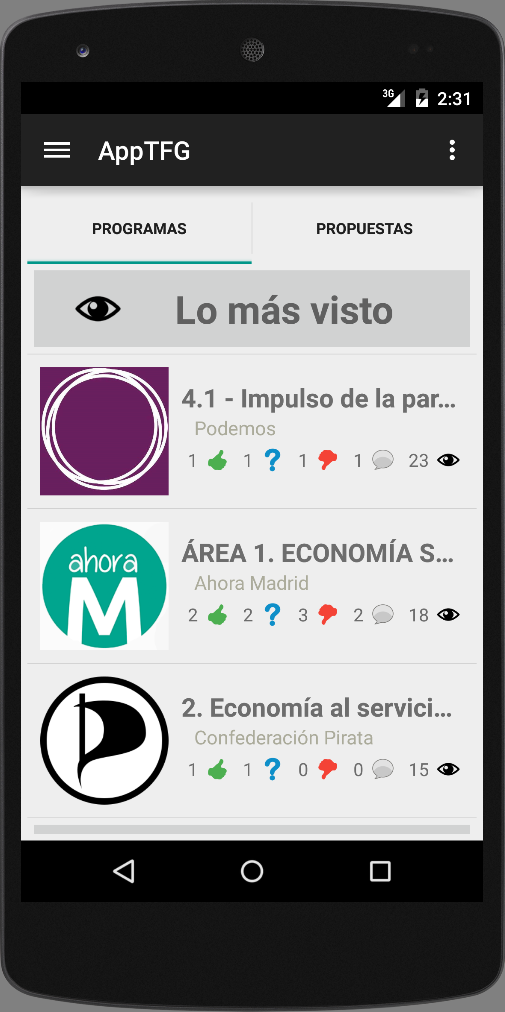
\includegraphics[keepaspectratio, scale=0.5]{Media/Captures/captTopSections.png}
\caption{Vista principal de secciones}
\label{fig:captTopSections}
\end{figure}

Dentro de cada sección podemos visualizar el contenido de la sección a la que referencia el programa, y tendremos la opción de valorarla de forma positiva o negativa. También añadimos la posibilidad de indicar que no se ha entendido la sección. Pues a la hora de leer una propuesta de gobierno ubicada en una sección del programa, bien nos puede gustar, disgustar o simplemente no haber entendido la idea y por ello no votarla de forma positiva o negativa.

\begin{figure}[H]
\centering
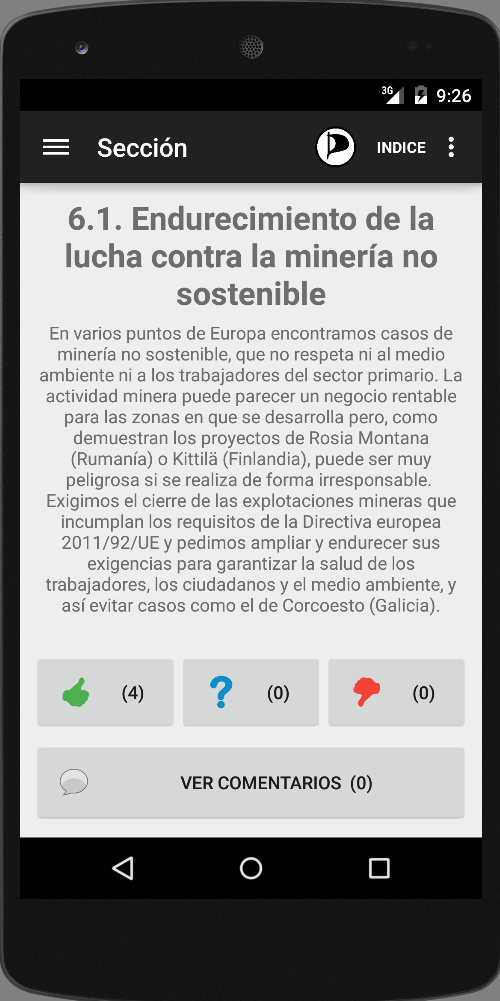
\includegraphics[keepaspectratio, scale=0.5]{Media/Captures/section.png}
\caption{Visualizando una sección}
\label{fig:captSection}
\end{figure}

Sin olvidarnos de la parte social, en cada sección podemos hacer comentarios para intentar debatir las ideas fundamentales que propone la sección. O incluso hacer referencia a una determinada frase o párrafo.

\subsubsection{Prototipo final}

\subsection{Análisis de Usabilidad}

Hablar de las reglas de oro, principios de diseño,...

HEURISTICA NIELSEN

\section{Implementación de DemoCritics}

METODOLOGIA GITHUB, CONTROL DE VERSIONES, GIT, REPARTO DE TAREAS: ANDROID - BACKEND, DEBUGGER consoloa-dispositivo, REVISIONES DE CODIGO, REVISION DE USABILIDAD.

\section{Evaluación con Usuarios}